\documentclass[12pt]{article}

\usepackage{fullpage}

\usepackage{amsmath}
\usepackage{url}
\usepackage{graphicx}
\usepackage{subfigure}
\usepackage{hyperref}

\bibliographystyle{plos2009}

\usepackage{xspace}
\newcommand{\dadi}{$\partial$a$\partial$i\xspace}
\newcommand{\bolddadi}{$\boldsymbol{\partial}$a$\boldsymbol{\partial}$i\xspace}
\newcommand{\Nref}{\ensuremath{N_\text{ref}}\xspace}
\newcommand{\ms}{\emph{ms}\xspace}
\usepackage{color}
\newcommand{\XXX}[1]{{\color{red}XXX:#1}}

\usepackage{listings}
\lstset{
basicstyle=\ttfamily,
language=Python,
showstringspaces=False,
aboveskip=0pt,
captionpos=b,
belowskip=0pt
}
\newcommand{\py}[1]{\lstinline[language=Python, showstringspaces=False]@#1@}
\newcommand{\ccode}[1]{\lstinline[language=C, showstringspaces=False]@#1@}
\newcommand{\shell}[1]{\lstinline[language=csh, showstringspaces=False]@#1@}
% For calibration, lines can be 60 characters long in
% lstlistings.
%\begin{lstlisting}
%*******************************************************
%\end{lstlisting}


\begin{document}
\title{\dadi user manual\\\normalsize  Corresponding to SVN $ $Revision$ $}
%\author{Ryan Gutenkunst}
\date{}
\maketitle

\tableofcontents

\clearpage

\section{Introduction}

Welcome to \dadi!

\dadi is a powerful software tool for simulating the joint frequency spectrum (FS) of genetic variation among multiple populations and employing the FS for population-genetic inference.
An important aspect of \dadi is its flexibility, particularly in model specification, but with that flexibility comes some complexity.
\dadi is not a GUI program, nor can \dadi be run usefully with a single command at the command-line; using \dadi requires at least rudimentary Python scripting.
Luckily for us, Python is a beautiful and simple language.
Together with a few examples, this manual will quickly get you productive with \dadi even if you have no prior Python experience.

\subsection{Getting help}

Please join the \py{dadi-announce} and \py{dadi-user} Google groups, available from the \dadi homepage: \url{http://dadi.googlecode.com}.
\py{dadi-announce} is a very low traffic list used only for alerting users to significant developments.
\py{dadi-user} is the preferred forum for asking questions and getting help.
Before posting a question, take a moment to look through the \py{dadi-user} archives (\url{http://groups.google.com/group/dadi-user}) to see if your question has already been addressed.
Additional detail on all the methods described here can be found in the API documentation, which is included with the source code distribution and available online at: \url{http://dadi.googlecode.com/svn/trunk/doc/api/index.html}.

\subsection{Helping us}

As we do our own research, \dadi is constantly improving.
Our philosophy is to include in \dadi any code we develop for our own projects that may useful to others.
Similarly, if you develop \dadi-related code that you think might be useful to others, please let us know so we can include it with the main distribution.

If you discover a bug in \dadi, please submit an issue on the \dadi website: \url{http://code.google.com/p/dadi/issues}.
Also, if you have particular needs that modification to \dadi may fulfill, please contact the developers and we may be able to help.

\section{Suggested workflow}

One of Python's major strengths is its interactive nature.
This is very useful in the exploratory stages of a project: for examining data and testing models.
If you intend to use \dadi's plotting commands, which rely on \py{matplotlib}, they you'll almost certainly want to install IPython, an enhanced Python shell that fixes several difficulties with interactive plotting using \py{matplotlib}.

My preferred workflow involves one window editing a Python script (e.g. \py{script.py}) and another running an IPython session (started as \py{ipython -pylab}).
In the IPython session I can interactively use \dadi, while I record my work in \py{script.py}.
IPython's \py{\%run script.py} magic command lets me apply changes I've made to \py{script.py} to my interactive session. 
(Note that you will need to reload other Python modules used by your script if you change them.)
Once I'm sure I've defined my model correctly and have a useful script, I run that from the command line (\py{python script.py}) for extended optimizations and other long computations.

Note that to access \dadi's functions, you will need to \py{import dadi} at the start of your script or interactive session.

If you are comfortable with Matlab, this workflow should seem very familiar.
Moreover the \py{numpy}, \py{scipy}, and \py{matplotlib} packages replicate much of Matlab's functionality.

\section{Importing data}

\dadi represents frequency spectra using \py{dadi.Spectrum} objects.
As described in section~\ref{sec:manip}, \py{Spectrum} objects are subclassed from \py{numpy.masked_array} and thus can be constructed similarly
The most basic way to create a \py{Spectrum} is manually:
\begin{lstlisting}
fs = dadi.Spectrum([0,100,20,10,1,0])
\end{lstlisting}
This creates a \py{Spectrum} object representing the FS from a single population, from which we have 5 samples.
(The first and last entries in \py{fs} correspond to mutations observed in zero or all samples. These are thus not polymorphisms, and by default \dadi masks out those entries so they are ignored.)

For nontrivial data sets, entering the FS manually infeasible, so we will focus on automatic methods of generating a \py{Spectrum} object.
The most direct way is to load a pre-generated FS from a file, using
\begin{lstlisting}
fs = dadi.Spectrum.from_file(filename)
\end{lstlisting}
The appropriate file format is detailed in the next section.

\subsection{Frequency spectrum file format}

\dadi uses a simple file format for storing the FS.
Each file begins with any number of comment lines beginning with \py{\#}.
The first non-comment line contains $P$ integers giving the dimensions of the FS array, where $P$ is the number of populations represented.
For a FS representing data from 4x4x2 samples, this would be \py{5 5 3}.
(Each dimension is one larger than the number of samples, because the number of observations can range, for example, from 0 to 4 if there are 4 samples, for a total of 5 possibilities.)
On the same line, the string \py{folded} or \py{unfolded} denoting whether or not the stored FS is folded.

The actual data is stored in a single line listing all the FS elements separated by spaces, in the order fs[0,0,0] fs[0,0,1] fs[0,0,2]\dots fs[0,1,0] fs[0,1,1]\dots.
This is followed by a single line giving the elements of the mask in the same order as the data, with \py{1} indicating masked and \py{0} indicating unmasked.

The file corresponding to the \py{Spectrum} \py{fs} can be written using the command:
\begin{lstlisting}
fs.to_file(filename)
\end{lstlisting}

\subsection{SNP data format}

As a convenience, \dadi includes several methods for generating frequency spectra directly from SNP data.
That relevant SNP file format is described here.
An large example can be found in the \py{examples/fs_from_data/data.txt} file included with the \dadi source distribution, and a small example is shown in Listing~\ref{lst:SNP_data}.

\begin{lstlisting}[caption={Example of SNP file format}, float, label={lst:SNP_data}]
Human Chimp Allele1 YRI  CEU  Allele2 YRI CEU Gene  Position
ACG   ATG   C       29   24   T       1   0   abcb1 289
CCT   CCT   C       29   23   G       3   2   abcb1 345
\end{lstlisting}

The data file begins with any number of comment lines that being with \py{#}.
The first parsed line is a column header line.
Whitespace is used to separate entries within the table, so no spaces are allowed within any entry.
Individual rows make be commented out using \py{#}.

The first column contains the in-group reference sequence at that SNP, including the flanking bases.
If the flanking bases are unknown, they can be denoted by \py{-}.
The header label is arbitrary.

The second column contains the aligned outgroup reference sequence at that SNP, including the flanking bases.
Unknown entries can be denoted by \py{-}.
The header label is arbitrary.

The third column gives the first segregating allele.
The column header must be exactly \py{Allele1}.

Then follows an arbitrary number of columns, one for each population, each giving the number of times Allele1 was observed in that population.
The header for each column should be the population identifier.

The next column gives the second segregating allele.
The column header must be exactly \py{Allele2}.

Then follows one column for each population, each giving the number of times Allele2 was observed in that population.
The header for each column should be the population identifier, and the columns should be in the same order as for the Allele1 entries.

Then follows an arbitrary number of columns which will be concatenated with \py{_} to assign a label for each SNP.

The \py{Allele1} and \py{Allele2} headers must be exactly those values because the number of columns between those two is used to infer the number of populations in the file.

\subsection{SNP data methods}

The method \py{Misc.make_data_dict} reads the above SNP file format to generate a Python data dictionary describing the data:
\begin{lstlisting}
dd = Misc.make_data_dict(filename)
\end{lstlisting}
From this dictionary, the method \py{Spectrum.from_data_dict} can be used to create a \py{Spectrum}.
\begin{lstlisting}
fs = Spectrum.from_data_dict(dd, pop_ids=['YRI', 'CEU'],
                             projections=[10, 12],
                             polarized=True)
\end{lstlisting}
The \py{pop_ids} argument specifies which populations to use to create the FS, and their order.
\py{projections} denotes the population sample sizes for the resulting FS.
Note that the total number of calls to Allele1 and Allele2 in a given population need not be the same for each SNP.
When constructing the Spectrum each SNP will be projected down to the requested number of samples in each population.
(Note that SNPs cannot be projected up, so SNPs without enough calls in any population will be ignored.)
\py{polarized} specifies whether \dadi should use outgroup information to polarize the SNPs.
If \py{polarized=True}, SNPs without outgroup information, or with that information \py{-} will be ignored.
If \py{polarized=False}, outgroup information will be ignored and the resulting \py{Spectrum} will be folded.

The method \py{Spectrum.from_data_dict_corrected} polarizes the SNPs using outgroup information and applies a statistical correction for multiple mutations described by Hernandez et al.~\cite{bib:Hernandez2007}.
Any SNPs without full trinucleotide ingroup and outgroup sequences will be ignored, as well as SNPs in which the flanking bases are not conserved between ingroup and outgroup, or in which the outgroup allele is not one of the segregating alleles.
The correction uses the expected number of substitutions per site, the trinucleotide mutation rate matrix, and a stationary trinucleotide distribution.
These are summarized in a table of misidentification probabilities that can be calculated using \py{Misc.make_fux_table}.
(It should also be possible to develop a correction using only the single-site transition matrix.
If this would be helpful, please contact the developers of \dadi.)

\section{Manipulating spectra}\label{sec:manip}

Frequency spectra are stored in \py{dadi.Spectrum} objects.
Computationally, these are a subclass of \py{numpy.masked_array}, so most of the standard array manipulation techniques can be used.
(In the examples here, I will typically be considering two-dimensional spectra, although all these features apply to higher-dimensional spectra as well.)

You can do arithmetic with \py{Spectrum} objects:
\begin{lstlisting}
fs3 = fs1 + fs2
fs2 = fs1 * 2
\end{lstlisting}
Note that most operations involving two \py{Spectrum} objects only make sense if they correspond to data with the same sample sizes.

Standard indexing and slicing operations work as well.
For example, to access the counts corresponding to 3 observations in population 1 and 5 observations in population 2, simply
\begin{lstlisting}
counts = fs[3,5]
\end{lstlisting}
More complicated slices are also possible.
The slice notation \py{:} indicates taking all corresponding entries.
For example, to access the slice of the \py{Spectrum} corresponding to entries with 2 derived allele observations in population 2, take
\begin{lstlisting}
slice = fs[:,2]
\end{lstlisting}

\subsection{Summary statistics}

The frequency spectrum encompasses many common summary statistics, and \dadi provides methods to calculate them from \py{Spectrum} objects.

\subsubsection{Single-population statistics}

Watterson's theta can be calculated as
\begin{lstlisting}
thetaW = fs.Watterson_theta()
\end{lstlisting}

The expected heterozygosity $\pi$ assuming random mating is
\begin{lstlisting}
pi = fs.pi()
\end{lstlisting}

Tajima's $D$ is
\begin{lstlisting}
D = fs.Tajima_D()
\end{lstlisting}

\subsubsection{Multi-population statistics}

The number of segregating sites $S$ is simply the sum of all entries in the FS (except for the absent-in-all and derived-in-all entries).
This can be calculated as
\begin{lstlisting}
S = fs.S()
\end{lstlisting}

Wright's $F_{ST}$ can be calculated as
\begin{lstlisting}
Fst = fs.Fst()
\end{lstlisting}
This estimate of Fst assumes random mating, because the FS does not store heterozygote.
Calculation is by the method of Weir and Cockerham~\cite{bib:Weir1984}.
For a single SNP, the relevant formula is at the top of page 1363.
To combine results between SNPs, we use the weighted average indicated by equation 10.

\subsection{Folding}

By default, \dadi considers the data in the \py{Spectrum} to be polarized, i.e. that the ancestral state of each variant is known.
In some cases, however, this may not be possible, and the FS must be \emph{folded}, indicating that only the minor allele frequency is known.
To fold a \py{Spectrum} object, simply
\begin{lstlisting}
folded = fs.fold()
\end{lstlisting}
The \py{Spectrum} object will record the fact that it has been folded, so that the likelihood and optimization machinery can automatically fold model spectra when the data are folded.

\subsection{Masking}

Finally, \py{Spectrum} arrays are \emph{masked}, i.e. certain entries can be set to be ignored.
Most typically, the ignored entries are the two corners: \py{[0,0]} and \py{[n1,n2]}, corresponding to variants observed in zero samples or in all samples.
More sophisticated masking is possible, however.
For example, if your calling algorithm is such that singletons in population 1 cannot be confidently called, you may want to ignore those entries of the FS in your analysis.
To do so, simply
\begin{lstlisting}
fs.mask[1,:] = True
\end{lstlisting}
Note that care must be taken when doing arithmetic with \py{Spectrum} objects that are masked in different ways.

\subsection{Marginalizing}

If one has a multidimensional \py{Spectrum} it may be useful to examine the marginalized \py{Spectrum} corresponding to a subset of populations.
To do so, use the \py{marginalize} method.
For example, consider a three-dimensional \py{Spectrum} consisting of data from populations A, B, and C.
To consider the marginal two dimensional spectrum for populations A and C, we need marginalize over population B.
\begin{lstlisting}
fsAC = fsABC.marginalize([1])
\end{lstlisting}
And to consider the marginal one-dimensional FS for population B, we marginalize over populations A and C.
\begin{lstlisting}
fsB = fsABC.marginalize([0,2])
\end{lstlisting}
Note that the argument to \py{marginalize} is a list of dimensions to marginalize over, \emph{indexed from 0}.

\subsection{Projection}

One can also project an FS down from a larger sample size to a smaller sample size.
Implicitly, this involves averaging over all possible re-samplings of the larger sample size data.
This is very often done in the case of missing data: if some sites could not be called in all individuals, one can set a lower bound on the number of successful calls necessary to include a SNP in the analysis; SNPs with more successful calls can then be projected down to that number of calls.

In \dadi, this is implemented with the \py{project} method.
For example, to project a two-dimensional FS down to sample sizes of 14 and 26, use
\begin{lstlisting}
proj = fs.project([14,26])
\end{lstlisting}

\subsection{Sampling}

One can simulate Poisson sampling from an FS using the \py{sample} method.
\begin{lstlisting}
sample = fs.sample()
\end{lstlisting}
Each entry in the \py{sample} output FS will have a Poisson number of counts, with mean given by the corresponding entry in \py{fs}.
If all sites are completely unlinked, this is a proper parametric bootstrap from your FS.

\subsection{Scrambling}

Occasionally, one may wish to ask whether the FS really represents samples from two populations or rather subsamples from a single population.
A rough check of this is to consider what the FS would look like if the population identifiers were scrambled amongst the individuals for whom you have data.
The \py{scramble} method will do this.
\begin{lstlisting}
scrambled = fs.scramble()
\end{lstlisting}
As an example, one could consider whether the FS for JPT and CHB shows evidence of differentiation between the two populations.
Note that this is an informal test, and we have not developed the theory to assign statistical significance to the results.
It is, nevertheless, a useful guide.

\section{Specifying a model}

A demographic model specifies population sizes and migration rates as a function of time, and it also includes discrete events such as population splittings and admixture.
Unlike many coalescent-based simulators, demographic models in \dadi are specified forward in time.
Also note that all population sizes within a demographic model are specified relative to some reference population size \Nref.

One important subtlety is that within the demographic model function, by default the mutation parameter $\theta = 4 \Nref \mu$ is set to 1.
This is because the optimal $\theta$ for a given model and set of data is trivial to calculate, so \dadi by default does this automatically in optimization (so-called ``multinomial'' optimization).
See Section~\ref{sec:fixed_theta} for how to fix theta to a particular value in a demographic model.

\subsection{Implementation}

Demographic models are specified by defining a Python function.
This function employs various methods defined by \dadi to specify the demography.

When defining a demographic function the arguments must be specified in a particular order.
The \emph{first} argument must be a list of free parameters that will be optimized.
The \emph{second} argument (usually called \py{ns}) must be a list of sample sizes.
The \emph{last} argument (usually called \py{pts}) must be the number of grid points used in the calculation.
Any additional arguments (between the second and last) can be used to pass additional non-optimized parameters, using the \py{func_args} argument of the optimization methods.
(See Listing~\ref{lst:new_world} for an example.)

The demographic model function tracks the evolution of $\phi$ the density of mutations within the populations at given frequencies.
This continuous density $\phi$ is approximated by its values on a grid of points, represented by the \py{numpy} array {phi}.
Thus the first step in a demographic model is to specify that grid:
\begin{lstlisting}
xx = dadi.Numerics.default_grid(pts)
\end{lstlisting}
Here \py{pts} is the number of grid points in each dimension for representing $\phi$.

All demographic models employed in \dadi must begin with an equilibrium population of non-zero size.
$\phi$ for such a population can be generated using the method \py{PhiManip.phi_1D}.
The most important parameter to this method is \py{nu}, which specifies the relative size of this ancestral population to the reference population.
Most often, the reference population is the ancestral, so \py{nu} defaults to 1.

Once we've created an initial $\phi$, we can begin to manipulate it.
First, we can split $\phi$ to simulate population splits.
This can be done using the methods \py{PhiManip.phi_1D_to_2D}, \py{PhiManip.phi_2D_to_3D_split_1}, and \py{PhiManip.phi_2D_to_3D_split_2}.
These methods take in an input $\phi$ of either one or two dimensions, and output a $\phi$ of one greater dimension, corresponding to addition of a population.
The added population is the last dimension of $\phi$.
For example, if \py{PhiManip.phi_2D_to_3D_split_1} is used, population 1 will split into populations 1 and 3.
\py{phi_2D_to_3D_admix} is a more advanced version of the \py{2D_to_3D} methods that incorporates admixture.
In this method, the proportions of pop 3 that are derived from pop 1 and pop 2 may be specified.

Direct admixture events can be specified using the methods \py{phi_2D_admix_1_into_2}, \py{phi_2D_admix_2_into_1}, \py{phi_3D_admix_1_and_2_into_3}, \py{phi_3D_admix_1_and_3_into_2}, and \py{phi_3D_admix_2_and_3_into_1}.
These methods do not change the dimensionality of $\phi$, but rather simulate discrete admixture events.
For example, \py{phi_2D_admix_1_into_2} can be used to simulate a large discrete influx of individuals from pop 1 into pop 2.
For example, this might model European (pop 1) admixture into indigenous Americans (pop 2).

Along with these discrete manipulations of $\phi$, we have the continuous transformations as time passes, due to genetic drift at different population sizes or migration.
This is handled by \py{Integration} methods, \py{Integration.one_pop}, \py{Integration.two_pops}, and \py{Integration.three_pops}.
Each of these methods must be used with a \py{phi} of the appropriate dimensionality.
\py{Integration.one_pop} takes two crucial parameters, \py{T} and \py{nu}.
\py{T} specifies the time of this integration and \py{nu} specifies the size of this population relative to the reference during this time period.
\py{Integration.two_pop} takes an integration time \py{T}, relative sizes for populations 1 and 2 \py{nu1} and \py{nu2}, and migration parameters \py{m12} and \py{m21}.
The migration parameter \py{m12} specifies the rate of migration \emph{from pop 2 into pop 1}.
It is equal to the fraction of individuals each generation in pop 1 that are new migrants from pop 2, times the 2\Nref.
\py{Integration.three_pops} is a straightforward extension of \py{two_pops} but now there are three population sizes and six migration parameters.

Note that for all these methods, the integration time \py{T} must be positive.
To ensure this, it is best to define your time parameters as the \emph{interval between} events rather than the absolute time of those events.
For example, a size change happened a time \py{Tsize} before a population split \py{Tsplit} in the past.

Importantly, population sizes and migration rates (and selection coefficients) may be functions of time.
This allows one to simulate exponential growth and other more complex scenarios.
To do so, simply pass a function that takes a single argument (the time) and returns the given variable.
The Python \py{lambda} expression is a convenient way to do this.
For example, to simulate a single population growing exponentially from size \py{nu0} to size \py{nuF} over a time \py{T}, one can do:
\begin{lstlisting}
nu_func = lambda t: nu0 * (nuF/nu0)**(t/T)
phi = Integration.one_pop(nu=nu_func, T=T)
\end{lstlisting}

Numerous examples are provided in Listings~\ref{lst:bottleneck} through~\ref{lst:new_world}.

\subsection{Units}
The units \dadi uses are slightly different than those used by some other programs, \ms in particular.

In \dadi, $\theta = 4 \Nref \mu$, as is typical.

Times are given in units of $2 \Nref$ generations.
This differs from \emph{ms}, where time is in units of $4 \Nref$ generations.
So to convert from a time in \dadi to a time in \emph{ms}, \emph{divide} by 2.

Migration rates are given in units of $M_{ij} = 2 \Nref m_{ij}$.
Again, this differs from \emph{ms}, where the scaling factor is $4 \Nref$ generations.
So to get equivalent migration ($m_{ij}$) in \ms for a given rate in \dadi, \emph{multiply} by 2.


\subsection{Fixed $\theta$}\label{sec:fixed_theta}

If you wish to set a fixed value of $\theta = 4 N_0 \mu$ in your analysis, that information must be provided to the initial $\phi$ creation function and the \py{Integration} functions.
For an example, see Listing~\ref{lst:fixed_theta}, which defines a demographic model in which $\theta$ is fixed to be 137 for derived population 1.
Derived pop 1 is thus the reference population for specifying all population sizes, so its size is set to 1 in the call to \py{Integration.two_pops}.
When fixing $\theta$, every \py{Integration} function must be told what the reference $\theta$ is, using the option \py{theta0}.
In addition, the methods for creating an initial $\phi$ distribution must be passed the appropriate value of $\theta$ using the \py{theta0} option.


\begin{lstlisting}[caption={\textbf{Bottleneck:} At time \py{TF} + \py{TB} in the past, an equilibrium population goes through a bottleneck of depth \py{nuB}, recovering to relative size \py{nuF}.}, float, label={lst:bottleneck}]
def bottleneck(params, ns, pts):
    nuB,nuF,TB,TF = params
    xx = Numerics.default_grid(pts)
    
    phi = PhiManip.phi_1D(xx)
    phi = Integration.one_pop(phi, xx, TB, nuB)
    phi = Integration.one_pop(phi, xx, TF, nuF)

    fs = Spectrum.from_phi(phi, ns, (xx,))
    return fs
\end{lstlisting}

\begin{lstlisting}[caption={\textbf{Exponential growth:} At time \py{T} in the past, an equilibrium population begins growing exponentially, reaching size \py{nu} at present.}, float]
def growth(params, ns, pts):
    nu,T = params

    xx = Numerics.default_grid(pts)
    phi = PhiManip.phi_1D(xx)

    nu_func = lambda t: numpy.exp(numpy.log(nu) * t/T)
    phi = Integration.one_pop(phi, xx, T, nu_func)

    fs = Spectrum.from_phi(phi, ns, (xx,))
    return fs
\end{lstlisting}

\begin{lstlisting}[caption={\textbf{Split with migration:} At time \py{T} in the past, two population diverge from an equilibrium population, with relative sizes \py{nu1} and \py{nu2} and with symmetric migration at rate \py{m}.}, float]
def split_mig(params, ns, pts):
    nu1,nu2,T,m = params

    xx = Numerics.default_grid(pts)

    phi = PhiManip.phi_1D(xx)
    phi = PhiManip.phi_1D_to_2D(xx, phi)

    phi = Integration.two_pops(phi, xx, T, nu1, nu2, m12=m, m21=m)

    fs = Spectrum.from_phi(phi, ns, (xx,xx))
    return fs
\end{lstlisting}

\begin{lstlisting}[caption={\textbf{Two-population isolation-with-migration:} The ancestral population splits into two, with a fraction \py{s} going into pop 1 and fraction \py{1-s} into pop 2. The populations then grow exponentially, with asymmetric migration allowed between them.}, float]
def IM(params, ns, pts):
    s,nu1,nu2,T,m12,m21 = params

    xx = Numerics.default_grid(pts)

    phi = PhiManip.phi_1D(xx)
    phi = PhiManip.phi_1D_to_2D(xx, phi)

    nu1_func = lambda t: s * (nu1/s)**(t/T)
    nu2_func = lambda t: (1-s) * (nu2/(1-s))**(t/T)
    phi = Integration.two_pops(phi, xx, T, nu1_func, nu2_func,
                               m12=m12, m21=m21)

    fs = Spectrum.from_phi(phi, ns, (xx,xx))
    return fs
\end{lstlisting}

\begin{lstlisting}[caption={\textbf{Out-of-Africa model from Gutenkunst (2009):} This model involves a size change in the ancestral population, a split, another split, and then exponential growth of populations 1 and 2. (The \py{from dadi import} line imports those modules from the \py{dadi} namespace into the local namespace, so we don't have to type \py{dadi.} to access them.)}, float]
from dadi import Numerics, PhiManip, Integration, Spectrum

def OutOfAfrica((nuAf, nuB, nuEu0, nuEu, nuAs0, nuAs, 
                 mAfB, mAfEu, mAfAs, mEuAs, TAf, TB, TEuAs),
                 (n1,n2,n3), pts):
    xx = Numerics.default_grid(pts)

    phi = PhiManip.phi_1D(xx)
    phi = Integration.one_pop(phi, xx, TAf, nu=nuAf)

    phi = PhiManip.phi_1D_to_2D(xx, phi)
    phi = Integration.two_pops(phi, xx, TB, nu1=nuAf, nu2=nuB, 
                               m12=mAfB, m21=mAfB)

    phi = PhiManip.phi_2D_to_3D_split_2(xx, phi)

    nuEu_func = lambda t: nuEu0*(nuEu/nuEu0)**(t/TEuAs)
    nuAs_func = lambda t: nuAs0*(nuAs/nuAs0)**(t/TEuAs)
    phi = Integration.three_pops(phi, xx, TEuAs, nu1=nuAf, 
                                 nu2=nuEu_func, nu3=nuAs_func, 
                                 m12=mAfEu, m13=mAfAs, m21=mAfEu,
                                 m23=mEuAs, m31=mAfAs, m32=mEuAs)

    fs = Spectrum.from_phi(phi, (n1,n2,n3), (xx,xx,xx))
    return fs
\end{lstlisting}

\begin{lstlisting}[caption={\textbf{Fixed $\boldsymbol{\theta}$:} A split demographic model function with a fixed value of $\theta$=137 for derived population 1. The free parameters are the sizes of the ancestral pop, \py{nuA}, and derived pop 2, \py{nu2}, (relative to derived pop 1), along with the divergence time \py{T} between the two derived pops.}, label={lst:fixed_theta}, float]
def fixed_theta((nuA, nu2, T), ns, pts):
    theta1 = 137
    
    xx = dadi.Numerics.default_grid(pts)
    
    phi = dadi.PhiManip.phi_1D(xx, nu=nuA, theta0=theta1)
    phi = dadi.PhiManip.phi_1D_to_2D(xx, phi)
    phi = dadi.Integration.two_pops(phi, xx, T, nu1=1, nu2=nu2,
                                    theta0=theta1)
                                    
    fs = dadi.Spectrum.from_phi(phi, ns, (xx,xx))
    return fs
\end{lstlisting}


\begin{lstlisting}[caption={\textbf{Settlement-of-New-World model from Gutenkunst (2009):} Because \dadi is limited to 3 simultaneous populations, we need to integrate out the African population, using \py{Numerics.trapz}. This model also employs a fixed $\theta$, and ancillary parameters passed in using the third argument.}, float, label={lst:new_world},basicstyle=\tt\footnotesize]
from dadi import Numerics, PhiManip, Integration, Spectrum

def NewWorld((nuEu0, nuEu, nuAs0, nuAs, nuMx0, nuMx,
              mEuAs, TEuAs, TMx, fEuMx), ns, 
             (theta0, nuAf, nuB, mAfB, mAfEu, mAfAs, TAf, TB),
             pts):
    xx = Numerics.default_grid(pts)

    phi = PhiManip.phi_1D(xx)
    phi = Integration.one_pop(phi, xx, TAf, nu=nuAf)

    phi = PhiManip.phi_1D_to_2D(xx, phi)
    phi = Integration.two_pops(phi, xx, TB, nu1=nuAf, nu2=nuB, 
                               m12=mAfB, m21=mAfB)

    # Integrate out the YRI population
    phi = Numerics.trapz(phi, xx, axis=0)

    phi = PhiManip.phi_1D_to_2D(xx, phi)
    nuEu_func = lambda t: nuEu0*(nuEu/nuEu0)**(t/(TEuAs+TMx))
    nuAs_func = lambda t: nuAs0*(nuAs/nuAs0)**(t/(TEuAs+TMx))
    phi = Integration.two_pops(phi, xx, TEuAs, 
                               nu1=nuEu_func, nu2=nuAs_func, 
                               m12=mEuAs, m21=mEuAs)
    phi = PhiManip.phi_2D_to_3D_split_2(xx, phi)

    # Initial population sizes for this stretch of integration
    nuEu0 = nuEu_func(TEuAs)
    nuAs0 = nuAs_func(TEuAs)
    nuEu_func = lambda t: nuEu0*(nuEu/nuEu0)**(t/TMx)
    nuAs_func = lambda t: nuAs0*(nuAs/nuAs0)**(t/TMx)
    nuMx_func = lambda t: nuMx0*(nuMx/nuMx0)**(t/TMx)
    phi = Integration.three_pops(phi, xx, TMx, 
                                 nu1=nuEu_func, nu2=nuAs_func, 
                                 nu3=nuMx_func,
                                 m12=mEuAs, m21=mEuAs,
                                 m23=mAsMx, m32=mAsMx)
    phi = PhiManip.phi_3D_admix_1_and_2_into_3(phi, fEuMx, 0,
                                               xx,xx,xx)

    fs = Spectrum.from_phi(phi, ns, (xx,xx,xx))
    # Apply our theta0. (All previous methods default to 
    # theta0=1.)
    return theta0*fs
\end{lstlisting}

\section{Simulation and fitting}

\subsection{Grid sizes and extrapolation}

To simulate the frequency spectrum, \dadi solves a partial differential equation, approximating the solution using a grid of points in population frequency space (the \py{phi} array).
Importantly, a single evaluation of the frequency spectrum with a fixed grid size is apt to be inaccurate, because computational limits mean the grid must be relatively coarse.
To overcome this, \dadi solves the problem at a series (typically 3) of grid sizes and extrapolates to an infinitely fine grid.
To transform the demographic model function you have created (call it \py{my_demo_func}) into a function that does this extrapolation, wrap it using a call to \py{Numerics.make_extrap_log_function}, e.g.:
\begin{lstlisting}
my_extrap_func = Numerics.make_extrap_log_func(my_demo_func)
\end{lstlisting}
Having done this, the final argument to \py{my_extrap_func} is now a \emph{sequence} of grid sizes, which will be used for extrapolation.
In our experience, good results are obtained by setting the smallest grid size slightly larger than the largest population sample size.
For example, if you have sample sizes of 16, 24, and 12 samples in the three populations you're working with, a good choice of grid sizes is probably \py{pts_l = [40,50,60]}.
This can be altered depending on your usage. For example, if you are fitting a complex slow model, it may speed up the analysis considerably to first run an optimization at small grid sizes (even less than the maximum number of samples).
This should get your parameter values approximately correct.
They can be refined by running another optimization with a finer grid.

A simulated frequency spectrum is thus obtained by calling
\begin{lstlisting}
model = my_extrap_func(params, ns, pts_l)
\end{lstlisting}
Here \py{ns} is the sequence of sample sizes for the populations in the model, \py{params} is the model parameters, and \py{pts_l} is the grid sizes.

\subsubsection{Grid choice}
As of version 1.5.0, the default grid in \dadi has points exponentially clustered toward $x=0$ and $x=1$.
This grid was suggested by Simon Gravel.
The parameter \py{crwd} controls how closely grid points crowd the endpoints of the interval.

We have performed some empirical investigations of the best value for \py{crwd}, although these results cannot be considered definitive.
We ran simulations for a variety of models and parameter values for a variety of sample sizes.
Denoting the largest sample size as \py{n}, we asked which value of \py{crwd} yielded the most accurate FS with \py{pts_l = [n, n+10, n+20]}.
Results are shown in Fig.~\ref{fig:best_crwd}.
It is evident that the best value for \py{crwd} is lower for smaller sample sizes.
The red lines are empirical functions which approximate the optimum.
These are implemented in \py{Numerics.estimate_best_exp_grid_crwd}.
Fig.~\ref{fig:consistent_crwd} demonstrates that the optimum value of \py{crwd} doesn't depend strongly on the number of grid points used for integration.
Unless you need absolute top performance, the default value of \py{crwd=8} will probably be sufficient.

\begin{figure}
\centering
\subfigure{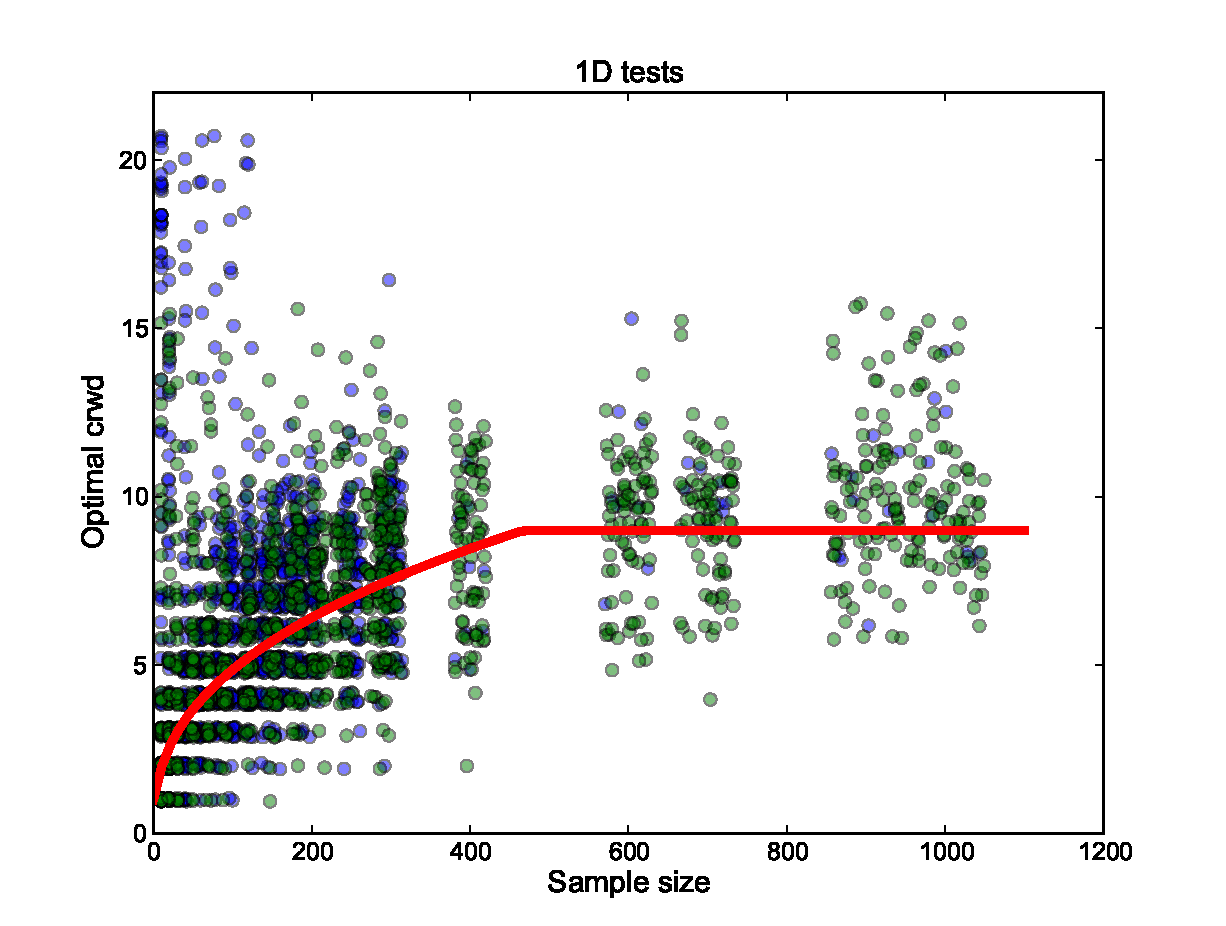
\includegraphics[scale=0.37]{opt_crwd_1d}}
\subfigure{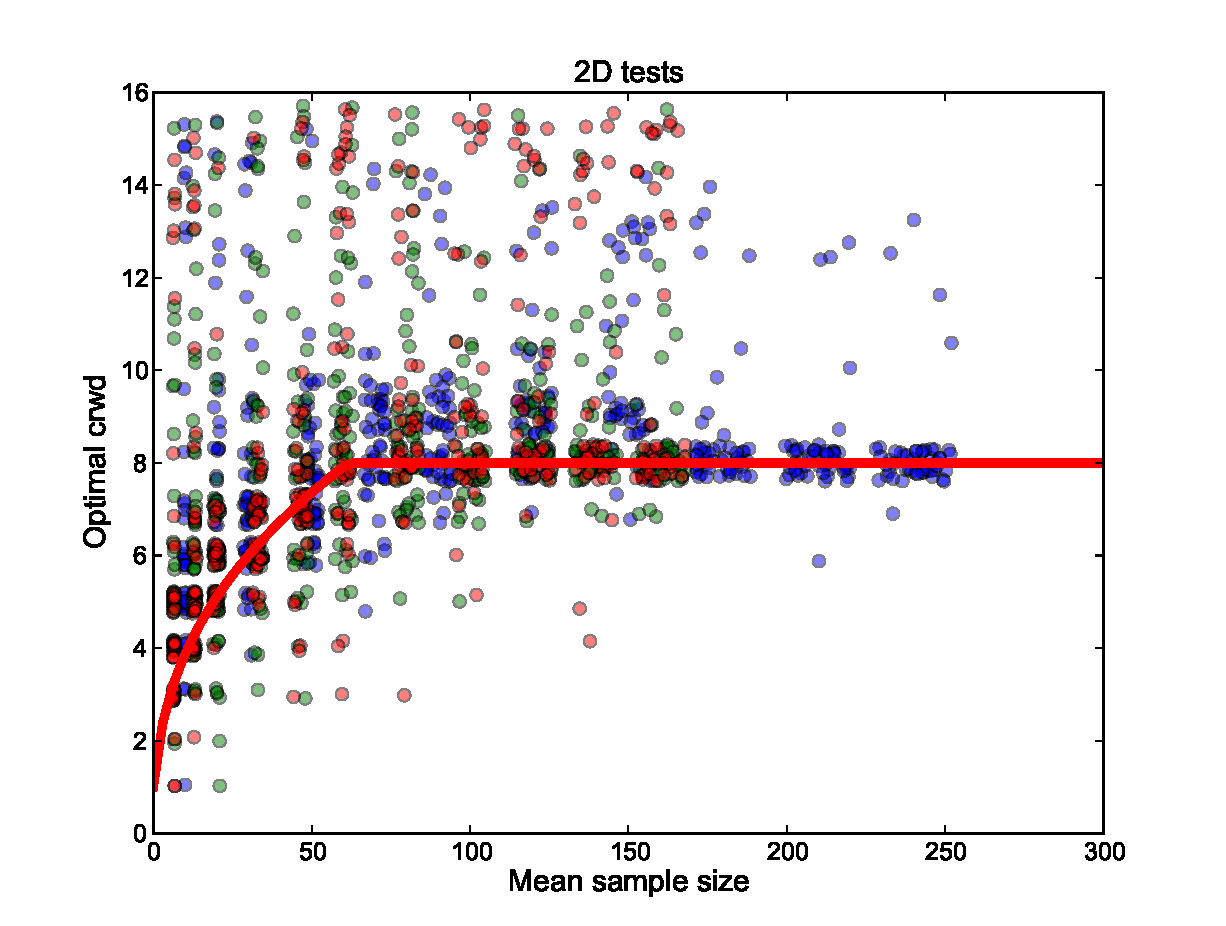
\includegraphics[scale=0.37]{opt_crwd_2d}}
\caption{\textbf{Empirical optimum values for \py{crwd}:} Each point represents the optimum value of \py{crwd} for a given model with a particular random choice of parameters.\label{fig:best_crwd}}
\end{figure}

\begin{figure}
\centering
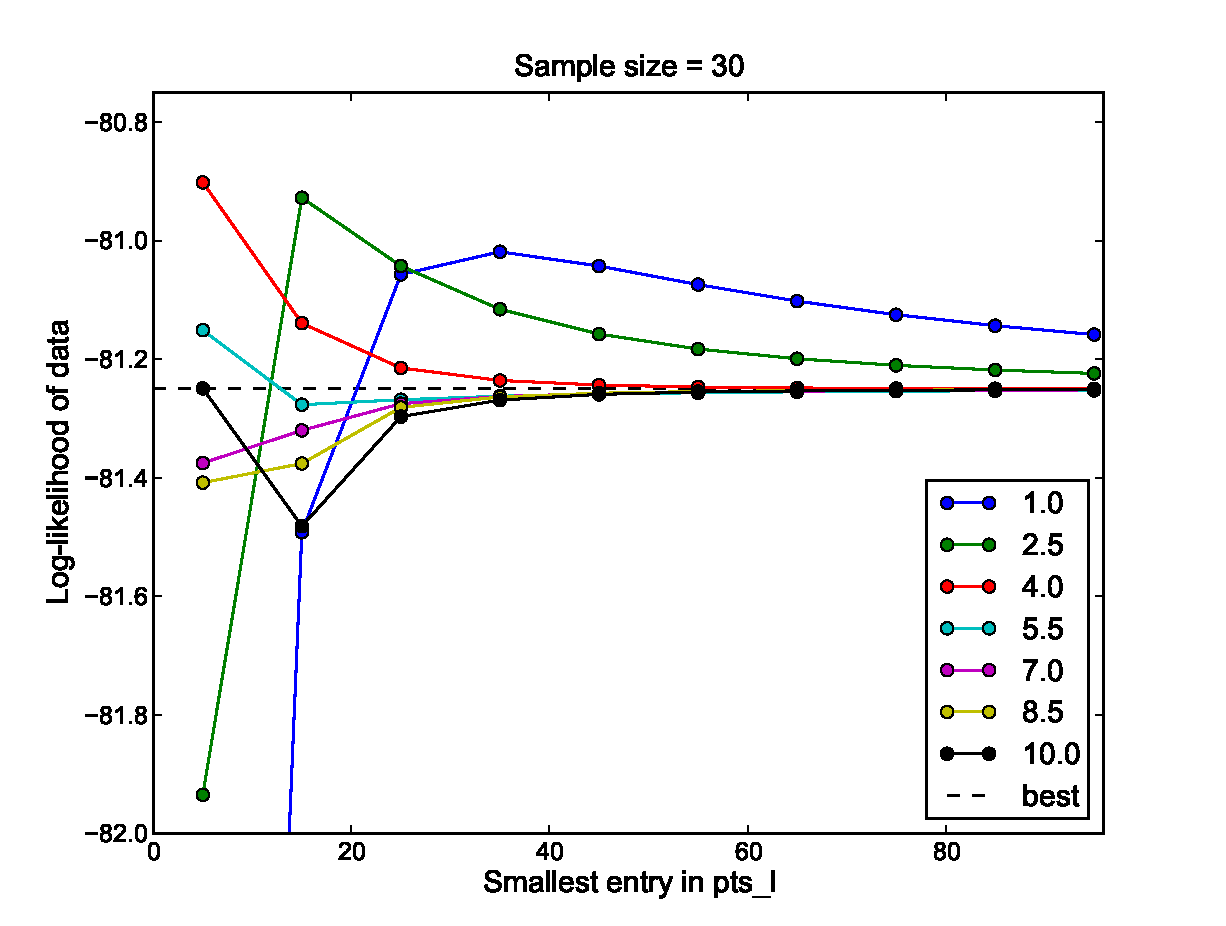
\includegraphics[scale=0.37]{consistent_crwd}
\caption{\textbf{Consistency of optimum \py{crwd} value:} For a one-dimensional system with 30 samples, the likelihood of a particular data set was calculated with \py{pts_l = [base, base+10, base+20]}, for varying \py{crwd} factors and values of \py{base}. In general, the optimum value of the \py{crwd} parameter does not depend on \py{base}.\label{fig:consistent_crwd}}
\end{figure}

\subsection{Likelihoods}

\dadi offers two complimentary ways of calculating the likelihood of the data FS given a model FS.
The first is the Poisson approach, and the second is the multinomial approach.

In the Poisson approach, the likelihood is the product of Poisson likelihoods for each entry in the data FS, given an expected value from the model FS.
This approach is relevant if $\theta_0$ is an explicit parameter in your demographic function.
Then the likelihood \py{ll} is
\begin{lstlisting}
ll = dadi.Inference.ll(model, data)
\end{lstlisting}

In the multinomial approach, before calculating the likelihood, \dadi will calculate the optimal $\theta_0$ for comparing model and data.
(It turns out that this is just $\theta_0 = \sum \text{data} / \sum \text{model}$.)
Because $\theta_0$ is so trivial to estimate given the other parameters in the model, it is most efficient for it \emph{not} to be an explicit parameter in the demographic function.
Then the likelihood \py{ll} is
\begin{lstlisting}
ll = dadi.Inference.ll_multinomial(model, data)
\end{lstlisting}
The optimal $\theta_0$ can be requested via
\begin{lstlisting}
theta0 = dadi.Inference.optimal_sfs_scaling(model, data)
\end{lstlisting}

\subsection{Fitting}

To find the maximum-likelihood model parameters for a given data set, \dadi employs non-linear optimization.
Several optimization methods are provided, as detailed in Section~\ref{sec:which_optimizer}.

\subsubsection{Parameter bounds}

In their exploration, the optimization methods typically try a wide range of parameter values.
For the methods that work in terms of log parameters, that range can be very wide indeed.
As a consequence, the algorithms may sometimes try parameter values that are very far outside the feasible range and that cause \emph{very} slow evaluation of the model FS.
Thus, it is important to place upper and lower bounds on the values they may try.
For divergence times and migration rates, large values cause slow evaluation, so it is okay to put the lower bound to 0 as long as the upper bound is kept reasonable.
In our analyses, we often set the upper bound on times to be 10 and the upper bound on migration rates to be 20.
For population sizes, very small sizes lead to very fast drift and consequently slow solution of the model equations; thus a non-zero lower bound is important, with the upper bound less so.
In our analyses, we often set the lower bound on population sizes to be $10^{-2}$ or $10^{-3}$ (i.e. \py{1e-2} or \py{1e-3}).

If your fits often push the bounds of your parameter space (i.e., results are often at the bounds of one or more parameters), this indicates a problem.
It may be that your bounds are too conservative, so try widening them.
It may also be that your model is misspecified or that there are unaccounted biases in your data.

\subsection{Fixing parameters}

It is often useful to optimize only a subset of model parameters.
A common example is doing likelihood-ratio tests on nested models.
The optional argument \py{fixed_params} to the optimization methods facilitates this.
As an example, if \py{fixed_params=[None,1.0,None,2.0]}, the first and third model parameters will be optimized, with the second and fourth parameters fixed to 1 and 2 respectively.
Note that when using this option, a full length initial parameter set \py{p0} should be passed in.

\subsection{Which optimizer should I use?}\label{sec:which_optimizer}

\dadi provides a multitude of optimization algorithms, each of which performs best in particular circumstances.

The two most-general purpose routines are the BFGS methods implemented in \py{dadi.Inference.optimize} and \py{dadi.Inference.optimize_log}.
These perform a local search from a specified set of parameters, using an algorithm which attempts to estimate the curvature of the likelihood surface.
However, these methods may have convergence problems if the maximum-likelihood parameters are at one or more of the parameter bounds.

\dadi also implements two L-BFGS-B methods, \py{dadi.Inference.optimize_lbfgsb} and \py{dadi.Inference.optimize_log_lbfgsb}.
These implement a variant of the BFGS method that deals much more efficiently with bounded parameter spaces.
If your optimizations are often hitting the parameter bounds, try using these methods.
Note that it is probably best to start with the vanilla BFGS methods, because the L-BFGS-B methods will always try parameter values at the bounds during the search.
This can dramatically slow model fitting.

We also provide a simplex (a.k.a. amoeba) method in terms of log parameters, implemented in \py{dadi.Inference.optimize_log_fmin}.
This method does not use derivative information, so it may be more robust than the BFGS-based methods, but it is much slower.

Finally, there is a simple grid search, implemented in \py{dadi.Inference.optimize_grid}.

Both BFGS and simplex are local search algorithms; thus they are efficient, but not guaranteed to find the global optimum.
Thus, it is important to run several optimizations for each data set, starting from different initial parameters.
If all goes well, multiple such runs will converge to the same set of parameters and likelihood, and this likelihood will the the highest found.
This is strong evidence that you have indeed found the global optimum.
To facilitate this, \dadi provides a method \py{dadi.Misc.perturb_params} that randomly perturbs the parameters passed in to generate a new initial point for the optimization.

%Note that the algorithm in \py{dadi.Inference.optimize} is typically more efficient than that in \py{dadi.Inference.optimize_log_fmin}.
%However, \py{optimize_log_fmin} can be more robust so if \py{optimize} is causing difficulty, you may consider trying \py{optimize_log_fmin}.


\section{Plotting}

For your convenience, \dadi provides several plotting methods.
These all require installation of the Python library \py{matplotlib}.

\subsection{Essential matplotlib commands}
To access additional, more general, methods for manipulating plots
\begin{lstlisting}
import pylab
\end{lstlisting}
In particular, the method \py{pylab.figure()} will create a new empty figure.

One quirk of \py{matplotlib} is that your plots may not show up immediately upon calling the plotting commands.
If they don't, a call to \py{pylab.show()} will pop them up.
If you are not running in IPython, this will cause Python to block, so do not place it in scripts you run from the command-line, unless it is the last line.

\subsection{1D comparison}

\begin{figure}
\centering
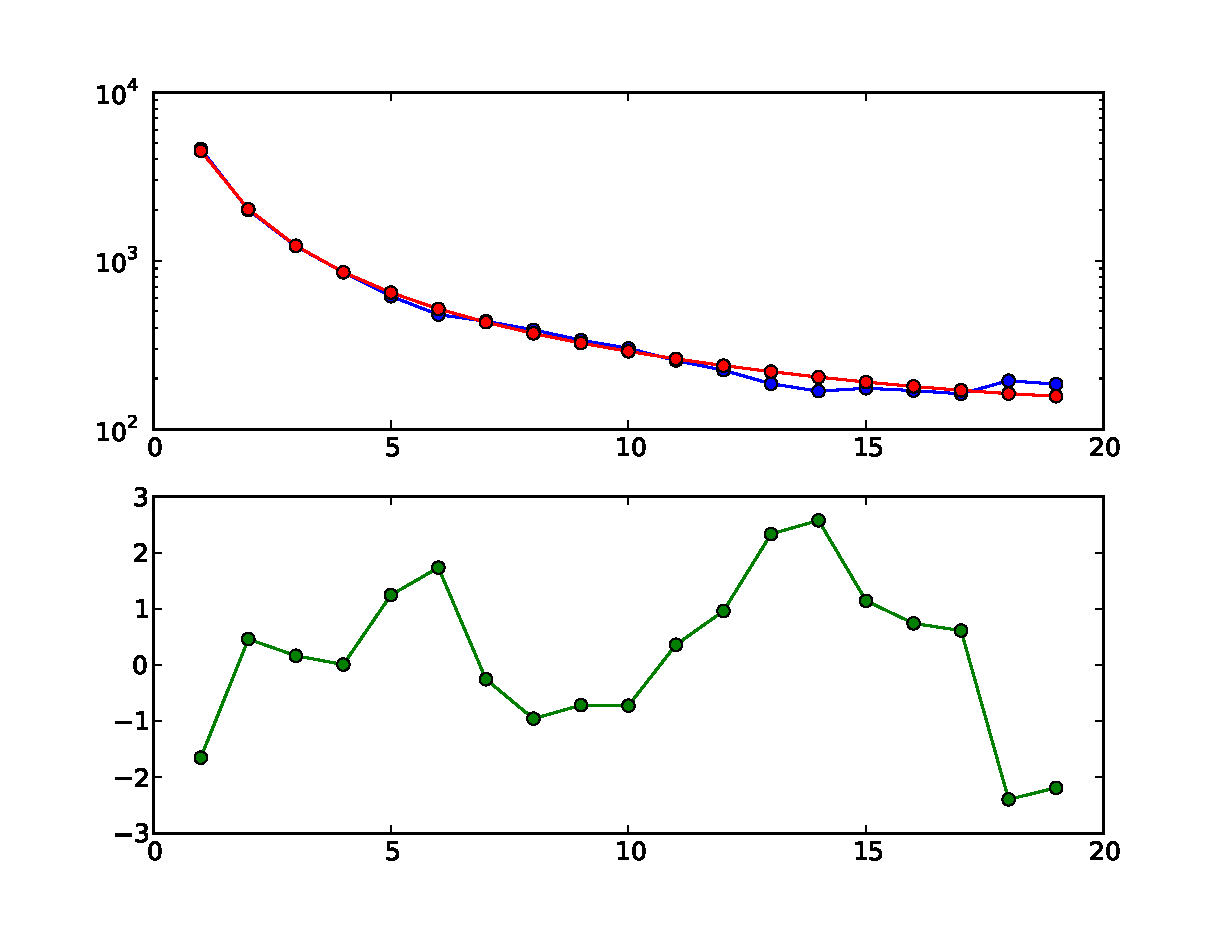
\includegraphics[scale=0.5]{1d_comp}
\caption{\textbf{1D model-data comparison plot:} In the top panel, the model is plotted in red and the data in blue. In the bottom panel, the residuals between model and data are plotted.\label{fig:1d_comp}}
\end{figure}

\py{dadi.Plotting.plot_1d_comp_Poisson} and \py{dadi.Plotting.plot_1d_comp_multinomial} plot a comparison between a one-dimensional model and data FS.
In the \py{_multinomial} method, the model is optimally scaled to match the data.
The plot is illustrated in Fig.~\ref{fig:1d_comp}.
The top plot shows the model and data frequency spectra, while the bottom shows the residuals between model and data.
The bottom plot shows the residuals between model and data; a positive residuals means the model predicts too many SNPs in that entry.
For an explanation of the residuals, see Section~\ref{sec:residuals}.

\subsection{2D spectra}

\begin{figure}
\centering
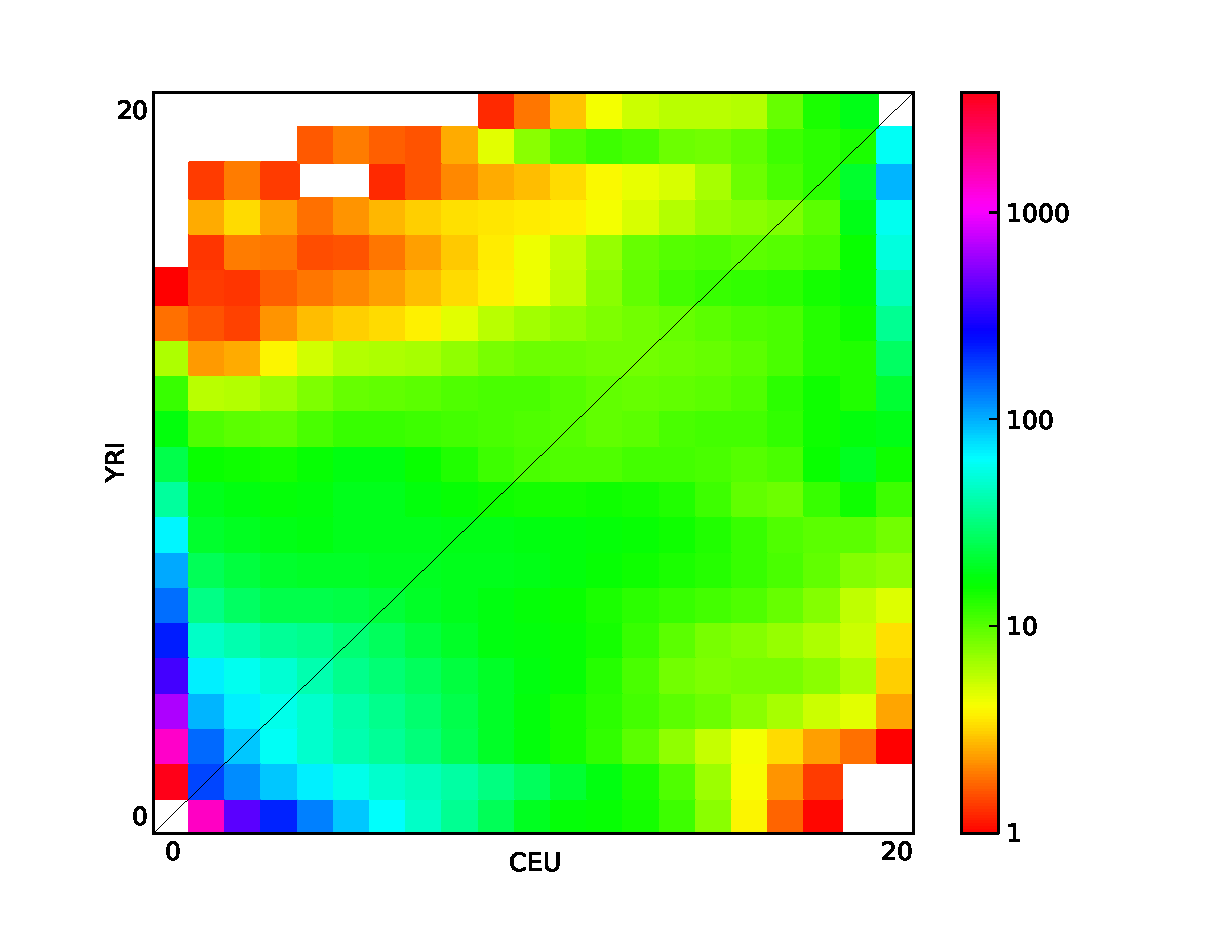
\includegraphics[scale=0.3]{2d_single}
\caption{\textbf{2D FS plot:} Each entry in the FS is colored according to the logarithm of the number of variants within it.\label{fig:2d_single}}
\end{figure}

\py{dadi.Plotting.plot_single_2d_sfs} will plot a single two-dimensional frequency spectrum, as a logarithmic colormap.
This is illustrated in Fig.~\ref{fig:2d_single}, which is the result of
\begin{lstlisting}
dadi.Plotting.plot_single_2d_sfs(data, vmin=1)
\end{lstlisting}
Here \py{vmin} indicates the minimum value to plot, because in a logarithmic plot 0 in the FS maps to minus infinity, which causes great difficulty in plotting.
Entires below the minimum (and masked entries) are plotted as white.

\subsection{2D comparison}

\begin{figure}
\centering
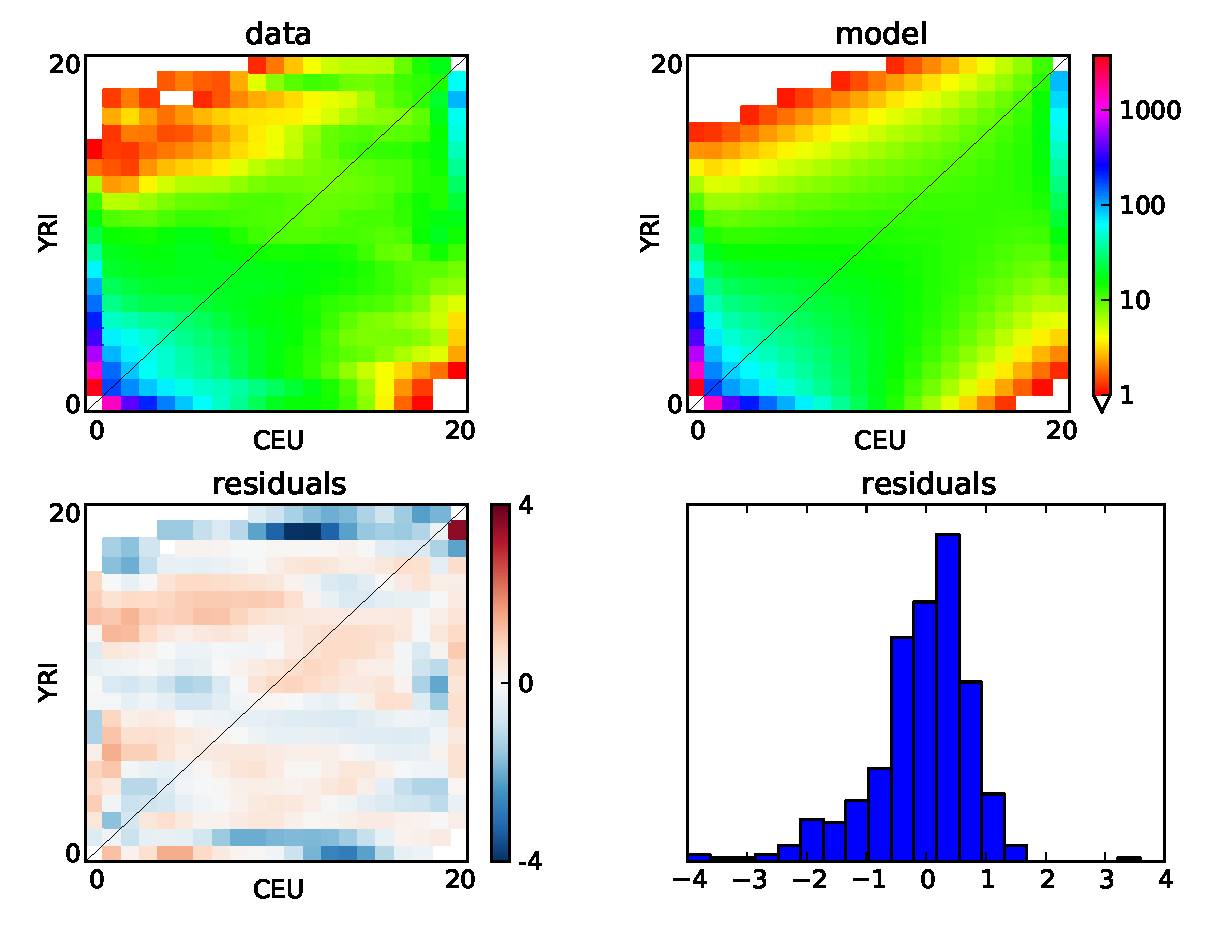
\includegraphics[scale=0.5]{2d_comp}
\caption{\textbf{2D model-data comparison plot:} The upper-left panel is the data, and the upper-right is the model. The lower two panels plot the residuals, and a histogram of the residuals.\label{fig:2d_comp}}
\end{figure}

\py{dadi.Plotting.plot_2d_comp_Poisson} and \py{dadi.Plotting.plot_2d_comp_multinomial} plot comparisons between 2D models and data.

\subsection{3D spectra}

Unfortunately, nice portable 3D plotting is difficult in Python.
We have developed a Mathematica script that will do such plotting (as in Fig.~2(A) of~\cite{bib:Gutenkunst2009}.)
Please contact the authors \py{dadi-user} and we will send you a copy.

\subsection{3D comparison}

\begin{figure}
\centering
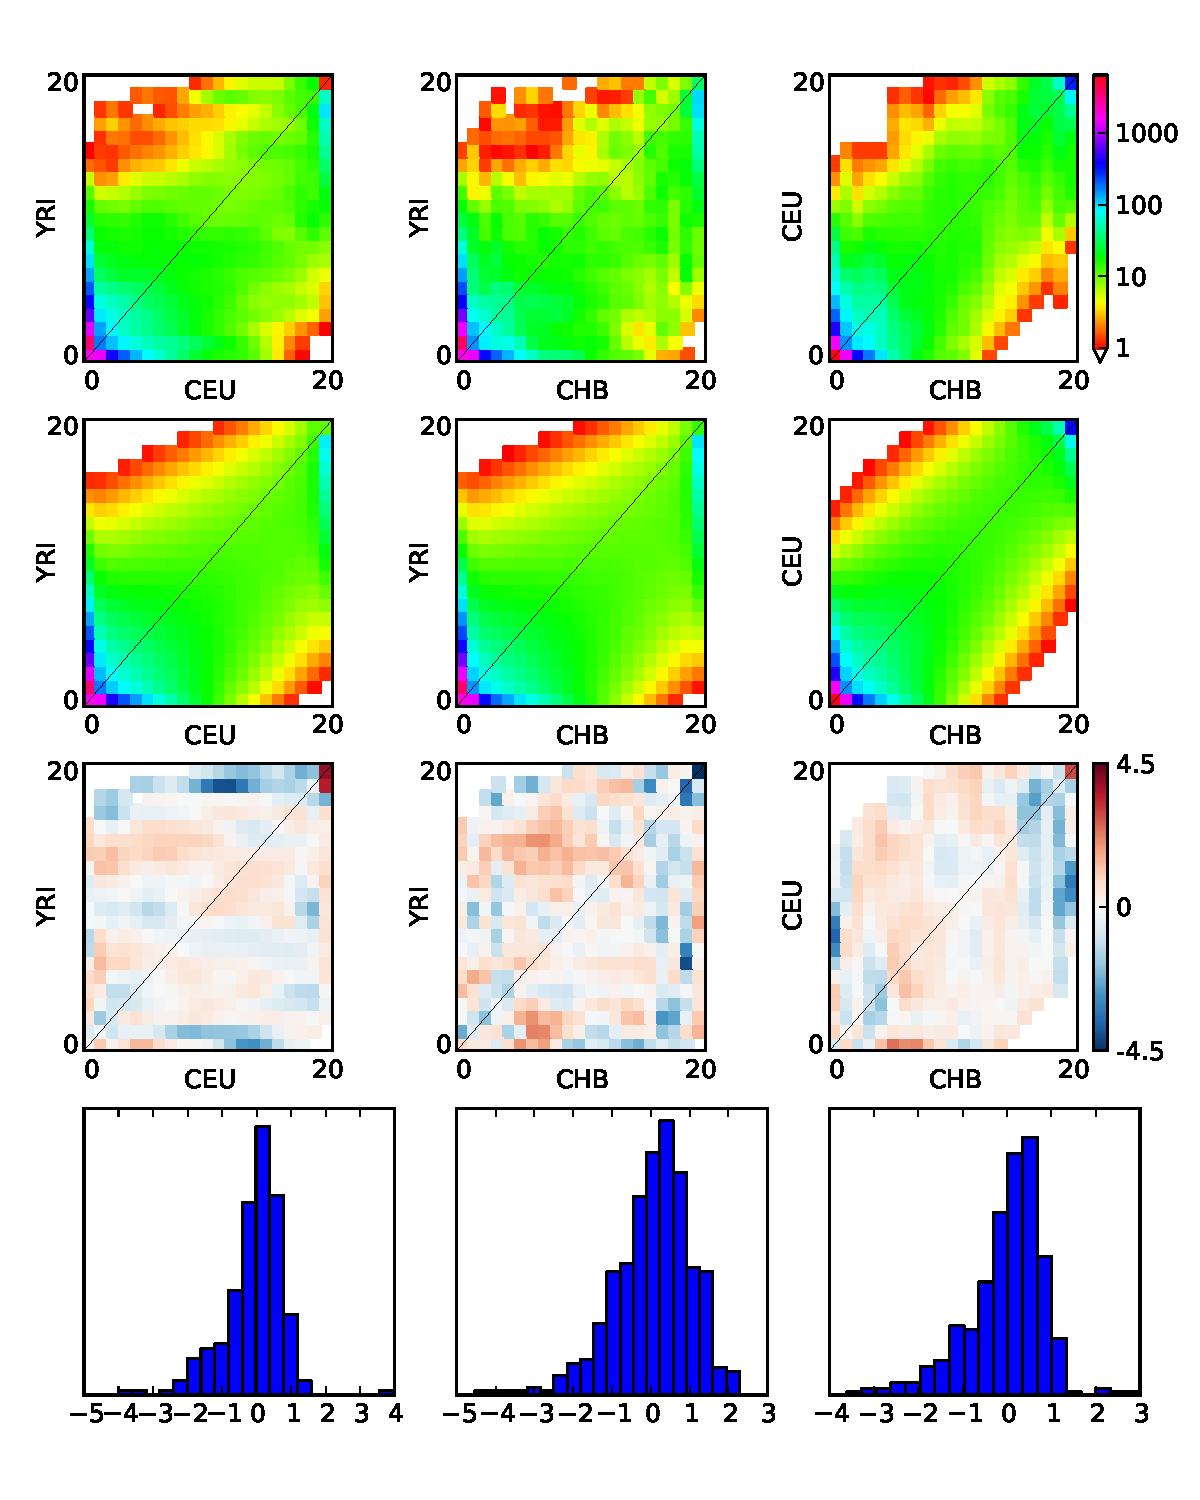
\includegraphics[scale=0.5]{3d_comp}
\caption{\textbf{3D model-data comparison plot:}\label{fig:3d_comp}}
\end{figure}

\py{dadi.Plotting.plot_3d_comp_Poisson} and \py{dadi.Plotting.plot_3d_comp_multinomial} plot comparisons between 3D models and data.
The comparison is based on the 3 2D marginal spectra.

\subsection{Residuals}\label{sec:residuals}

The residuals are the properly normalized differences between model and data.
Normalization is necessary, because the expected variance in each entry increase with the expected value of that entry.
Two types of residuals are supported, Poisson and Anscombe.

The Poisson residual is simply
\begin{equation}
\text{residual} = (\text{model} - \text{data})/\sqrt{\text{model}}.
\end{equation}
Note, however, that this residual is not normally distributed when the expected value (model entry) is small.

The Anscombe residual is
\begin{equation}
\text{residual} = \frac{3}{2} \, \frac{(\text{model}^\frac{2}{3} - \text{model}^{-\frac{1}{3}}/9) - (\text{data}^\frac{2}{3} - \text{data}^{-\frac{-1}{3}}/9)}{\text{model}^\frac{1}{6}}.
\end{equation}
These residuals are more normally distributed than the Poisson residuals when expected values are small~\cite{bib:Pierce1986}.

\section{Bootstrapping}

Because \dadi's likelihood function treats all variants as independent, and they are often not, standard likelihood theory should not be used to estimate parameter uncertainties are significance levels for hypothesis tests.
To do such tests, one can bootstrap.
For estimating parameter uncertainties, one can use a nonparameteric bootstrap, i.e. sampling with replacement from independent units of your data (genes or chromosomes) to generate new data sets to fit.
For hypothesis tests, the parametric bootstrap is preferred.
This involves using a coalescent simulator (such as \ms) to generate simulated data sets.
Care must be taken to simulate the sequencing strategy as closely as possible.

\subsection{Interacting with \ms}

\dadi provides several methods to ease interaction with \ms.
The method \py{Spectrum.from_ms_file} will generate an FS from \ms output.
The method \py{Misc.ms_command} will generate the command line for \ms corresponding to a particular simulation.
As an example:
\begin{lstlisting}
import os

core = "-n 1 -n 2 -ej 0.3 2 1"
command = dadi.Misc.ms_command(theta=1000, ns=(20,20), core, 1000,
                               recomb=0.3)
ms_fs = dadi.Spectrum.from_ms_file(os.popen(command))
\end{lstlisting}
Here the \py{os.popen} command lets us read the \ms output straight from the command, without writing an intermediate file to disk.
If you'd like to actually write the file, you could do
\begin{lstlisting}
os.system("%s > temp.msout" % command)
ms_fs = dadi.Spectrum.from_ms_file("temp.msout")
\end{lstlisting}

\section{Installation}

\subsection{Dependencies}

\dadi depends on a number of Python libraries. The absolute dependencies are
\begin{itemize}
\item Python, version $\geq$ 2.5 (but not Python 3)
\item NumPy, version $\geq$ 1.2.0
\item SciPy, version $\geq$ 0.6.0
\end{itemize}
It is also recommended that you install
\begin{itemize}
\item matplotlib, version $\geq$ 0.98.1
\item IPython, version $\geq$ 0.10
\end{itemize}
For 3D plotting, it is also suggested that you install
\begin{itemize}
\item MayaVi2
\end{itemize}

The easiest way to obtain all these dependencies is to install \href{http://www.enthought.com/products/epd.php}{Enthought's Python Distribution}, which is \href{http://www.enthought.com/products/edudownload.php}{free for academic use}.

\subsection{Binary packages}

The easiest way to get \dadi is to download and run one of the binary installers.
Note that we still suggest downloading the source distribution to have access to tests, examples, and documentation.
(The installation of Python that ships with OS X may not be detected by the binary installer.
You'll typically be better off installing one of the \py{python.org} distributions.)
Note that installers are specific to the minor version of Python. For example, a 2.5 installer will work on 2.5.1 and 2.5.4, but not on 2.6.
If you need a binary installer for a particular version of Python, please ask on the \py{dadi-users} mailing list.

\subsection{Installing from source}

\dadi can be easily installed from source code, as long as you have \py{gcc} installed. (On OS X, you'll need to install the Developer Tools to get \py{gcc}.) To do so, first unpack the source code tarball, \py{unzip dadi-<version>.zip}.
In the \py{dadi-<version>} directory, run \py{sudo python setup.py install}.
This will compile the C modules \dadi uses and install those plus all \dadi Python files in your Python installation's \py{site-packages} directory.
A (growing) series of tests can be run in the \py{tests} directory, via \py{python run_tests.py}

\subsubsection{Windows}

Installing \py{gcc} on Windows is somewhat troublesome. If you are running Python 2.6, \dadi can also be compiled on Windows if you have Microsoft Visual Studio 2008. There is a free ``Express'' version which includes the compiler available at \url{http://www.microsoft.com/express/Downloads/}.

\section{Frequently asked questions}

\begin{enumerate}
\item What does the message \py{WARNING:Inference:Model is < 0 where data is not masked.} mean?

This warning comes from the likelihood calculation function.
It indicates that the model frequency spectrum has negative values that are trying to be compared with data.
Negative values in the frequency spectrum are nonsense, so this most likely indicates numerical difficulties.
If you're running an optimization, occasional warnings like this likely not a problem.
The optimization explores a wide range of parameter values, most of which are bad fits.
If these errors crop up for parameter values that will be a bad fit anyways, the errors won't change the final result.
On the other hand, if you are re getting these warnings near good-fitting sets of parameters, you'll need to fix them.
There are two possible causes, and thus two possible solutions.

\begin{enumerate}
\item The negative values might be arising from the extrapolation process (over different grid sizes).
In this case, replace any calls to \py{Numerics.make_extrap_func} to \py{Numerics.make_extrap_log_func}.
This will do the extrapolation based on the logarithms of the value in the frequency spectrum, guaranteeing positive results.

\item The negative values might be arising from calculating an individual spectrum (for a fixed grid size).
This typically only happens in cases of very rapid exponential growth.
In this case, you can try a finer grid size (increase the elements of the \py{pts_l} list) or smaller time steps.
The time step is set by the call to \py{dadi.Integration.set_timescale_factor(pts_l[-1], factor=10)}.
To shorten the time step, increase \py{factor}.
First try shortening the time step, as this will typically increase computation time less than increasing the grid size.
\end{enumerate}

\item I'm projecting my data down to a smaller frequency spectrum. What sample sizes should I project down to?

At this time, we have not done any formal power testing to judge the optimal level of projection, but we do have a rule-of-thumb.
As you project down to smaller sample sizes, more SNPs can be used in constructing the FS (because they have
enough successful calls).
However, as you project downward, some SNPs will ``disappear'' from the FS because they get partially projected down
to 0 observations in all the populations.
Our rule of thumb is to use the projection that maximizes the number of segregating SNPs.
The number of segregating SNPs can be calculated as \py{fs.S()}.

\item Can I use a likelihood-ratio-test to decide whether allowing a parameter to be non-zero yields a statistically significantly better model? (For example, migration versus no migration.)

Yes, although assigning significance values can be computationally intensive.
\dadi calculates a composite likelihood, which assumes all SNPs in the data are independent.
This doesn't bias parameter inference for neutral models~\cite{bib:Wiuf2006}, but if your SNPs are actually linked, the standard likelihood-ratio test will be anti-conservative, i.e. it will reject the more complex model more often that it should.

To overcome this, you need to calculate the null distribution, i.e. what improvements in likelihood would you expect if there really were no migration in the data, but your model included migration?
To do this, generate simulated data sets with a coalescent simulator under your best-fit model without migration, replicating as closely as possible your sequencing strategy (size and linkage between sequenced regions).
Then fit each data set using the no-migration model, and the migration model.
The resulting distribution of likelihood differences is the null distribution, i.e. if there really is no migration, how much does
adding the migration parameter improve the likelihood (because you're better fitting noise)?
Compare the improvement from the real data with this null distribution to assign a p-value.

\end{enumerate}

%\begin{lstlisting}[caption={Dork}, float]
%blah blah
%\end{lstlisting}

%\thebibliography
\bibliography{popgen}


\end{document}